%%%%%%%%%%%%%%%%%%%%%%%%%%%%%%%%%%%%%%%%%
% Structured General Purpose Assignment
% LaTeX Template
%
% This template has been downloaded from:
% http://www.latextemplates.com
%
% Original author:
% Ted Pavlic (http://www.tedpavlic.com)
%
% Note:
% The \lipsum[#] commands throughout this template generate dummy text
% to fill the template out. These commands should all be removed when
% writing assignment content.
%
%%%%%%%%%%%%%%%%%%%%%%%%%%%%%%%%%%%%%%%%%

%----------------------------------------------------------------------------------------
%	PACKAGES AND OTHER DOCUMENT CONFIGURATIONS
%----------------------------------------------------------------------------------------

\documentclass{article}
\setcounter{tocdepth}{4}
\setcounter{secnumdepth}{4}
\usepackage{fancyhdr} % Required for custom headers
\usepackage{lastpage} % Required to determine the last page for the footer
\usepackage{extramarks} % Required for headers and footers
\usepackage{graphicx} % Required to insert images
\usepackage{lipsum} % Used for inserting dummy 'Lorem ipsum' text into the template
\usepackage{url}
\usepackage{amsmath}
\usepackage{amssymb}
\usepackage{arydshln}
\usepackage{mathtools}
\usepackage{breqn}
\usepackage{fixltx2e}
\usepackage{indentfirst} 
\graphicspath{ {images/} }
\usepackage{bm}

% Margins
\topmargin=-0.45in
\evensidemargin=0in
\oddsidemargin=0in
\textwidth=6.5in
\textheight=9.0in
\headsep=0.25in

\linespread{1.1} % Line spacing

% Set up the header and footer
\pagestyle{fancy}
\lhead{\hmwkClass\ : \hmwkTitle} % Top center header
\rhead{\firstxmark} % Top right header
\lfoot{\lastxmark} % Bottom left footer
\cfoot{} % Bottom center footer
\rfoot{Page\ \thepage\ } % Bottom right footer
\renewcommand\headrulewidth{0.4pt} % Size of the header rule
\renewcommand\footrulewidth{0.4pt} % Size of the footer rule

\setlength\parindent{2em} % Indentation for paragraphs


%----------------------------------------------------------------------------------------
%	NAME AND CLASS SECTION
%----------------------------------------------------------------------------------------

\newcommand{\hmwkTitle}{Kalman Filtering for an Inverted Pendulum Final Report} % Assignment title
\newcommand{\hmwkDueDate}{Wednesday,\ June\ 6,\ 2018} % Due date
\newcommand{\hmwkClass}{MAE\ 298} % Course/class
\newcommand{\hmwkClassTime}{} % Class/lecture time
\newcommand{\hmwkClassInstructor}{Professor Lin} % Teacher/lecturer
\newcommand{\hmwkAuthorName}{Jordan McCrone, Sarah O'Meara, Peng Chen} % Your name

%----------------------------------------------------------------------------------------
%	TITLE PAGE
%----------------------------------------------------------------------------------------

\title{
\vspace{2in}
\textmd{\textbf{\hmwkClass:\ \hmwkTitle}}\\
\normalsize\vspace{0.1in}\large{Due\ on\ \hmwkDueDate}\\
\vspace{0.1in}\large{\textit{\hmwkClassInstructor\ \hmwkClassTime}}\\
\vspace{3in}
}

\author{\textbf{\hmwkAuthorName}}
\date{} % Insert date here if you want it to appear below your name

%----------------------------------------------------------------------------------------
%	USER COMMANDS
%----------------------------------------------------------------------------------------

\newcommand{\matr}[1]{\bm{#1}}     % ISO complying version

%----------------------------------------------------------------------------------------
\begin{document}

\maketitle

%----------------------------------------------------------------------------------------
%	TABLE OF CONTENTS
%----------------------------------------------------------------------------------------

%\setcounter{tocdepth}{1} % Uncomment this line if you don't want subsections listed in the ToC

\newpage
\tableofcontents
\listoffigures
\listoftables
\newpage

\section{Examples}
Test as seen in \cite{kane}

Example superscript JACO\textsuperscript{2} Example citation \cite{weisz2017assistive}

\begin{figure}[h!]
	\centering
	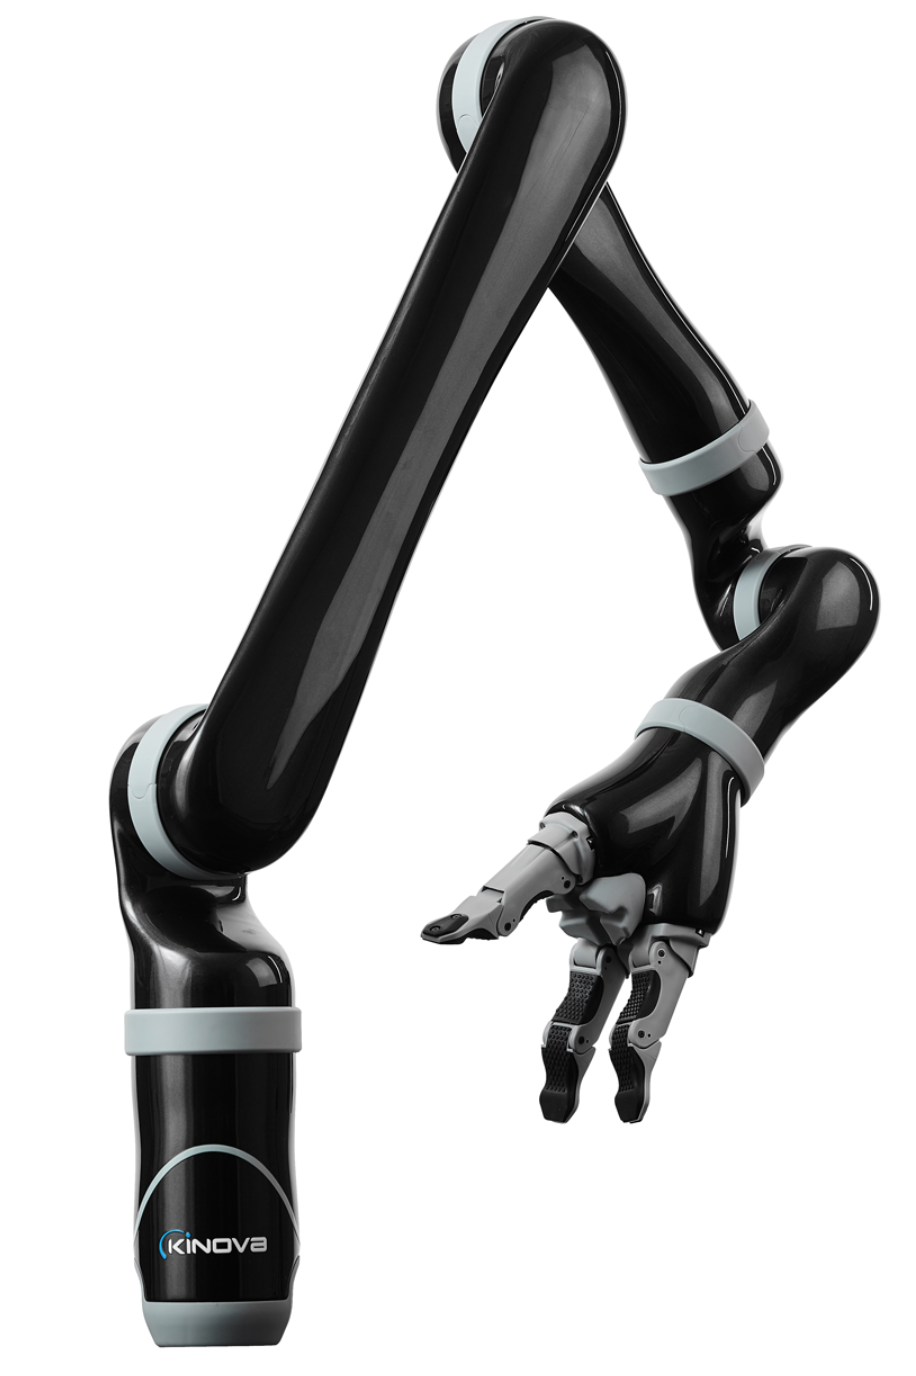
\includegraphics[width=5cm,keepaspectratio]{kinova.png}
	\caption{JACO\textsuperscript{2} 6-DOF Manipulator}
	\label{fig:diagram1}
\end{figure}

Example Figure \ref{fig:diagram1} Example symbols $\epsilon$. Example table

\begin{table}[h!]
\centering
\begin{tabular}{ |c |c  |c |c |c  |c  |c |}
\hline
	 i & 1 & 2 & 3 & 4 & 5 & 6 \\ \hline
	 a\textsubscript{i} & 0 & d\textsubscript{2} & 0 & 0 & 0 & 0 \\ \hline
	 $\alpha$\textsubscript{i}  & -90 & 0 & -90 & 90 & -90 & 0 \\ \hline
	 $\theta$\textsubscript{i} & $\theta$\textsubscript{1} & $\theta$\textsubscript{2} & $\theta$\textsubscript{3} & $\theta$\textsubscript{4} & $\theta$\textsubscript{5} & $\theta$\textsubscript{6} \\ \hline
	 s\textsubscript{i} & -d\textsubscript{1} & 0 & $\epsilon$\ &  d\textsubscript{3} + d\textsubscript{4} & 0 & d\textsubscript{5} + d\textsubscript{6} \\ \hline
\end{tabular}
\caption{D-H Parameters}
\label{table:1}
\end{table}

Example matrix with no equation number
\[
A_{1} = 
\begin{bmatrix}
	C\theta_{1} & 0 & -S\theta_{1} & 0 \\
	S\theta_{1} & 0 & C\theta_{1} & 0  \\
	0 & -1 & 0 & -d_{1} \\
	0 & 0 & 0 & 1 \\ 
\end{bmatrix}
\]

\section{Introduction}

 The inverted pendulum is a common system that has been well-studied in dynamics and controls.  The identifying characteristic of these systems is that the center of mass is above the pivot point resulting in an inherently unstable system.  Examples of inverted pendulum systems range from humans, where the feet are considered the pivot point, to the self-balancing Segway.  These systems are nonlinear and require a feedback control loop and state estimation in order to balance or stabilize the system, such that the center of mass remains directly above the pivot point.  Any displacement from this configuration will result in the center of mass moving to a new equilibrium at the lowest potential energy.  The center of mass can be repositioned above the pivot point by a control system that applies a restorative force.  It is critical to provide the controller with accurate state estimations in order to calculate the appropriate restorative force.  Inaccurate state estimation can destabilize the system leading to large oscillations or an undesirable state, such as the Segway falling onto the ground.

 This project used a pole on a cart model as an inverted pendulum system and investigated the use of different estimators: the Kalman Filter (KF), the Extended Kalman Filter, and the Unscented Kalman Filter.  Since the KF is used for linearized systems, it is hypothesized that its performance will degrade at larger angles as the small angle approximation will be used to linearize the equations of motion.  The project also tested the use of a single sensor and two sensors, and it is expected that two sensors will yield a more accurate estimation of the states.  Finally, this project evaluated the RMSE (root mean square error) and run time across estimators (KF, EKF, UKF) with different tuning.  The following sections discuss the system, state space models, test cases, results, and conclusions.

\section{Derivation of Continuous State Space Model}

The model used for our analysis is a 2 degree-of-freedom system (see Figure \ref{fig:sys_diagram}). It includes a rigid pole that has a single axis of rotation, and is attached to the cart with a pin-joint. The cart has a single translational axis corresponding to the ground plane. The underlying assumptions of this model are:

\begin{enumerate}
\item No friction between the ground and the cart wheels
\item No friction between cart and pole
\item Pole is a uniform, slender rod
\item Air resistance is negligible
\item Cart remains in contact with the ground
\item Ground is flat and level
\end{enumerate}

\begin{figure}[h!]
	\centering
	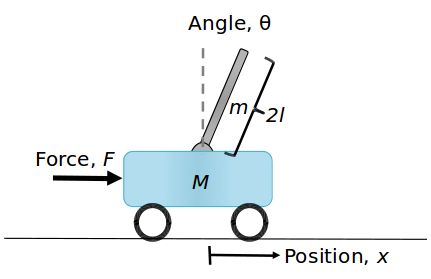
\includegraphics[width=5cm,keepaspectratio]{SystemDiagram.png}
	\caption{System Diagram}
	\label{fig:sys_diagram}
\end{figure}

 Using the above assumptions, we derived the non-linear equations of motion using Newton's second law.
\begin{equation}
\begin{aligned}
\frac{4}{3}l \ddot{\theta} &= g \sin \theta - \cos \theta \ddot{x} \\
(M+m)\ddot{x} &= F + ml \theta^2 \sin\theta -ml\ddot{\theta}\cos\theta
\end{aligned}
\label{eq:EOM_nonlinear}
\end{equation}
These can be rearranged into the nonlinear continuous-time first-order system of equations
\begin{equation}
\begin{aligned}
\matr{\dot{x}} &= \matr{f}(\matr{x},u),\quad  \matr{x} = \begin{bmatrix}
	x \\
	\dot{x} \\
	\theta \\
	\dot{\theta} \\
\end{bmatrix} \\
\matr{\dot{x}} &= \begin{bmatrix}
	\dot{x} \\
	\ddot{x} \\
	\dot{\theta} \\
	\ddot{\theta} \\
\end{bmatrix} = \begin{bmatrix}
\dot{x} \\
\frac{F+ml\dot{\theta}^2\sin\theta}{M+m} -\frac{ml\cos\theta}{m+M}\frac{mgl\sin\theta- \frac{ml}{M+m} F\cos\theta -\frac{m^2l^2}{m+M}\dot{\theta}^2\sin\theta\cos\theta}{J+ml^2-\frac{m^2l^2}{M+m}\cos^2 \theta } \\[6pt]
\dot{\theta} \\
\frac{mgl\sin\theta - \frac{ml}{M+m} F\cos\theta -\frac{m^2l^2}{m+M}\dot{\theta}^2\sin\theta\cos\theta}{J+ml^2-\frac{m^2l^2}{M+m}\cos^2 \theta }
\end{bmatrix}
\end{aligned}
\end{equation}
In order to implement a linear Kalman Filter, we will need to linearize these equations. Since the unstable portion of the system is directly related to the angle of the pole, it is our desire to keep the pole at the vertical position of 0$^\circ$. Therefore, this is the angle is the one about which we want to linearize, and this is often called the "small angle approximation." This first-order truncation of the trigonometric Taylor series expansions results in the following substitutions to our nonlinear equations:
\begin{align*}
\sin \theta &\approx \theta \\
\cos \theta &\approx 1 \\
\dot{\theta}^2 &\approx 0
\end{align*}
Making these substitutions and rearranging the equations into matrix form results in the Linear State Space Model:
\begin{equation}
\begin{bmatrix}
	\dot{x} \\
	\ddot{x} \\
	\dot{\theta} \\
	\ddot{\theta} \\
\end{bmatrix} = \begin{bmatrix}
0 & 1 & 0 & 0 \\
0 & 0 & -\frac{-m^2l^2g}{\gamma} & 0 \\
0 & 0 & 0 & 1\\
0 & 0 & \frac{(M+m)mgl}{\gamma} & 0
\end{bmatrix} \begin{bmatrix}
	x \\
	\dot{x} \\
	\theta \\
	\dot{\theta} \\
\end{bmatrix}  + \begin{bmatrix}
0 \\
\frac{J+ml^2}{\gamma} \\
0 \\
-\frac{ml}{\gamma}
\end{bmatrix} F
\label{eq:ss_continuous}
\end{equation}
where 
\begin{align*}
\gamma &= J(M+m)+mMl^2 \\
J &= \frac{1}{3}ml^2
\end{align*}
The original intention when applying a Kalman filter to this system was that we would measure just one of the states directly, and use these measurements to estimate the pole angle. We discovered that the only state output that measurement that resulted in a full-rank observability matrix $\mathcal{O}$ was the measurement of cart position. However, we ran into problems (See "Controllability and Observability", Appendix), and determined that a better estimator could be built if we measured two states, one of which was the cart position. Therefore, we also chose to measure pole angular rate, resulting in the output equation
\begin{align}
y = \begin{bmatrix}
1 & 0 & 0 & 0 \\
0 & 0 & 0 & 1
\end{bmatrix} \begin{bmatrix}
	x \\
	\dot{x} \\
	\theta \\
	\dot{\theta} \\
\end{bmatrix}
\label{eq:1output}
\end{align}
Equations \ref{eq:ss_continuous} and \ref{eq:1output} are representations of the familiar linear state-space form
\begin{equation}
\begin{aligned}
\matr{\dot{x}} &= \matr{A}\matr{x} + \matr{B}u \\
\matr{y} &= \matr{C}\matr{x}
\end{aligned}
\end{equation}
The state that is imperative for accurate measurement is the pole angle. In this pursuit, we want to select the highest accuracy sensors, within a reasonable range of cost. We looked at a few sensors, and \\

Based on this information, we selected an initial process and model noise of
\begin{equation}
\begin{aligned}
w_k \sim N(0,\sigma_w^2) \\
v_k \sim N(0,\sigma_v^2)
\end{aligned}
\end{equation}
\subsection{Description of System and Assumptions}
\subsection{System Parameters}

\begin{equation}
\matr{x} = 
\begin{bmatrix}
	x \\
	\dot{x} \\
	\theta \\
	\dot{\theta} \\
\end{bmatrix}
\label{xMatrix}
\end{equation}

\begin{equation}
\beta = \dfrac{4}{3} - \dfrac{m}{M+m}
\end{equation}

\begin{equation}
\matr{A} = 
\begin{bmatrix}
	1 & \tau & 0 & 0 \\
	0 & 1 & \dfrac{-gm\tau}{(M+m)\beta} & 0 \\
	0 & 0 & 1 & \tau \\
	0 & 0 & \dfrac{g\tau}{l\beta} & 1 \\
\end{bmatrix}
\label{aMatrix}
\end{equation}

\begin{equation}
\matr{A} = 
\begin{bmatrix}
	1 & \tau & 0 & 0 \\
	0 & 1 & \dfrac{-gm\tau}{(M+m)\beta} & 0 \\
	0 & 0 & 1 & \tau \\
	0 & 0 & \dfrac{g\tau}{l\beta} & 1 \\
\end{bmatrix}
\label{aMatrix}
\end{equation}

\section{Estimators and Resulting Discretized State Space Models}
\subsection{Kalman Filter (KF)}
\subsection{Extended Kalman Filter (EKF)}
\subsection{Unscented Kalman Filter (UKF)}

\section{Methodology}

\section{Results}
\subsection{Offline Results}
\subsection{Online Results}

\section{Conclusions}

\section{References}

%\cite{*}
\bibliography{references}{}
\bibliographystyle{ieeetr}

\pagebreak
\section{Appendices}
\subsection{Controllability and Observability}
\label%latex
To check observability $\mathcal{O}$ and controllability $\mathcal{C}$, we constructed their respective matrices from the linear discrete time state space model using
\begin{equation}
\mathcal{C} = \begin{bmatrix}
B & AB & A^2B & A^3B
\end{bmatrix} = \begin{bmatrix}
    0.0003 &   0.0009  &  0.0015   & 0.0021 \\
    0.0300  &  0.0300  &  0.0300   & 0.0301 \\
   -0.0005   &-0.0014  & -0.0023   &-0.0033 \\
   -0.0456  & -0.0461  & -0.0471   &-0.0485
\end{bmatrix}
\end{equation}
A quick check with MATLAB using the command rank($\mathcal{C}$) tells us $\mathcal{C}$ is rank(4), which by the textbook definition makes this system controllable. \\

Our initial attempt at using a Kalman filter with just one measurement (cart position) was not working very well. We then determined to check the observability matrix $\mathcal{O}$, defined as
\begin{equation}
\mathcal{O} = \begin{bmatrix}
C \\
CA \\
CA^2 \\
CA^3
\end{bmatrix}
\end{equation}
This matrix was also full rank, which was perplexing. Professor Lin then suggested that we check the condition number of the observability matrix. Using the MATLAB command cond(), we evaluated cond($\mathcal{O}$) = $6.67e-5$, which suggests that the observability matrix is almost singular. This was the source of some of our problems in implementing our state estimators. Based on this information, we attempted to add another sensor at the pole angular rate. After doing this, the condition number of the observability matrix was $60.437$, a much more reasonable number.
\ref{eq:EOM_nonlinear}
\subsubsection{junk}
\begin{dmath}
	\hat{z_{6}} \times \vec{r_{6}} = \left[\begin{matrix}0\\0\\0\end{matrix}\right]
\end{dmath}


\end{document}
